% 本章节是介绍 RISC-V的
\section{计算机组成与设计——基于RISC-V}
依据 David A. Patterson 的著作 Computer Prganization and Design RISC-V Edition \cite{Computer_Organization_and_Design_riscv}以及浙江大学刘鹏博导的公开课\cite{Computer_Organization_and_Design_ZJU} 作为参考理解,这里主要讨论 RISC-V 的指令集以及流
水线。

\subsection{指令表示方法与指令格式}
其实抛开课堂上 PPT 枯燥的概念,如果把计算机比作一个正在说话的人,那么指令就是那个人每句话中的每一个单词,而指令集就是全部词汇所构成的词汇表,也正是有指令集的存在,计算机才能实现“开口说话”与沟通,接下来介绍一下 RISC-V 的常用指令。

\subsubsection{R指令}
\textbf{R指令}的作用是用于处理处理器内部的寄存器与寄存器之间算数运算产生的。

一条R型指令的格式划分如图\ref{fig:R-Format_Instruction_Layout}所示,一个 R 型指令可以被划分成为 6 个域,其中31-25 这 7bit 宽的是功能码 7,24-20 这 5 位是源寄存器 2,19-15 这 5 位是源寄存器 1,14-12这 3bit 宽的是功能码 3,11-7 这 5bit 宽的目的寄存器 rd,6-0 这 7 位宽的操作码 (部分规定了该指令是什么指令)。

\begin{figure}[htbp]
    \centering
    \def\svgwidth{\columnwidth}
    \import{./figs/RISC-V/指令表示/R-Format_Instruction_Layout/}{R-Format_Instruction_Layout.pdf_tex}
    \caption{R型指令格式的划分,其中每个域中的文字表示该域的名称;域上的数字表示,该域的起始与终止位置;每个域下面的数字,表示每个域所占据的bit位数}
    \label{fig:R-Format_Instruction_Layout}
\end{figure}
% \begin{figure}[htbp]
%   \centering %居中显示
%   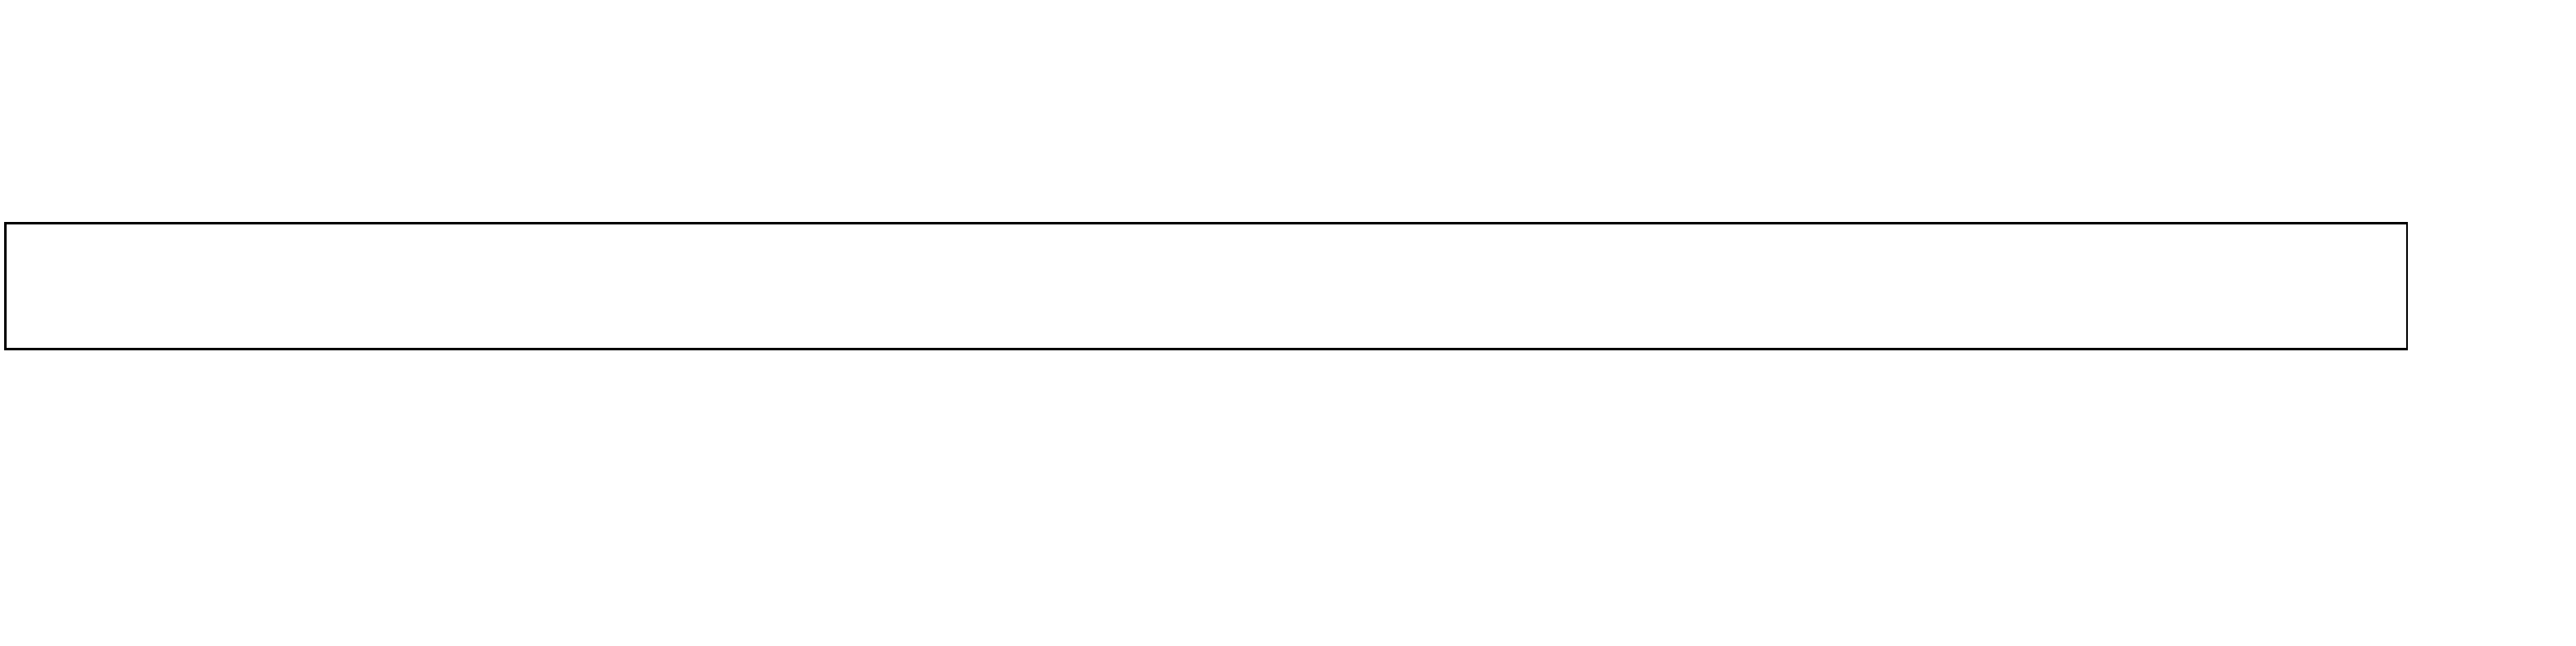
\includegraphics[width=0.8 \textwidth]{figs/RISC-V/指令表示/R-Format_Instruction_Layout.eps}
%   \caption{R型指令格式的划分\\ 其中每个域中的文字表示该域的名称;域上的数字表示,该域的起始与终止位置;每个域下面的数字,表示每个域所占据的bit位数}
%   \label{fig:R-Format_Instruction_Layout} %设置图形引用名称
% \end{figure}

所有 R 指令的 opcode 部分都是 2 进制数:0110011,funct7 与 funct3 是和 opcode 结合起来一起使用的,三者组合一起规定指令的操作。

rs1,rs2 是源寄存器 (Source Rggister), 是用于暂存源操作数的地址;
rd 是目的寄存器(Destination Rggister),指定接收结果值的寄存器编号,这三个寄存器都存放 5 位无符号整数 (对应十进制 25 = 32),对应 0 ~31 的通用寄存器中的其中一个。

\subsubsection{I指令}
\textbf{I指令}是用于寄存器与立即数之间算数运算和读取产生的。

如果换成是我自己设计指令架构,我很有可能将操作寄存器,操作数用一个指令全部实现,但是我看了别人的设计之后发现我以前的想法中存在一个问题,就是指令中的位长,比方说 R 指令的源地址和目的地址才 5bit,最多就能表示 10 进制的 32 位,那要是操作数字就显得有些有限;但是如果你把指令中的位长加长的话,就会造成可以表示的 10 进制数太多,但是寄存器就 32 了,造成不必要的浪费。

所以,I 型指令可以在 R 型指令的基础上做一些稍微的改动即可,如图\ref{fig:R_I}

\begin{figure}[htbp]
    \centering
    \def\svgwidth{\columnwidth}
    \import{./figs/RISC-V/指令表示/R_I/}{R_I.pdf_tex}
    \caption{I型指令就是把R型指令的前两个域合并成一个了12位的有符号数}
    \label{fig:R_I}
\end{figure}

% \begin{figure}[htbp]
%   \centering %居中显示
%   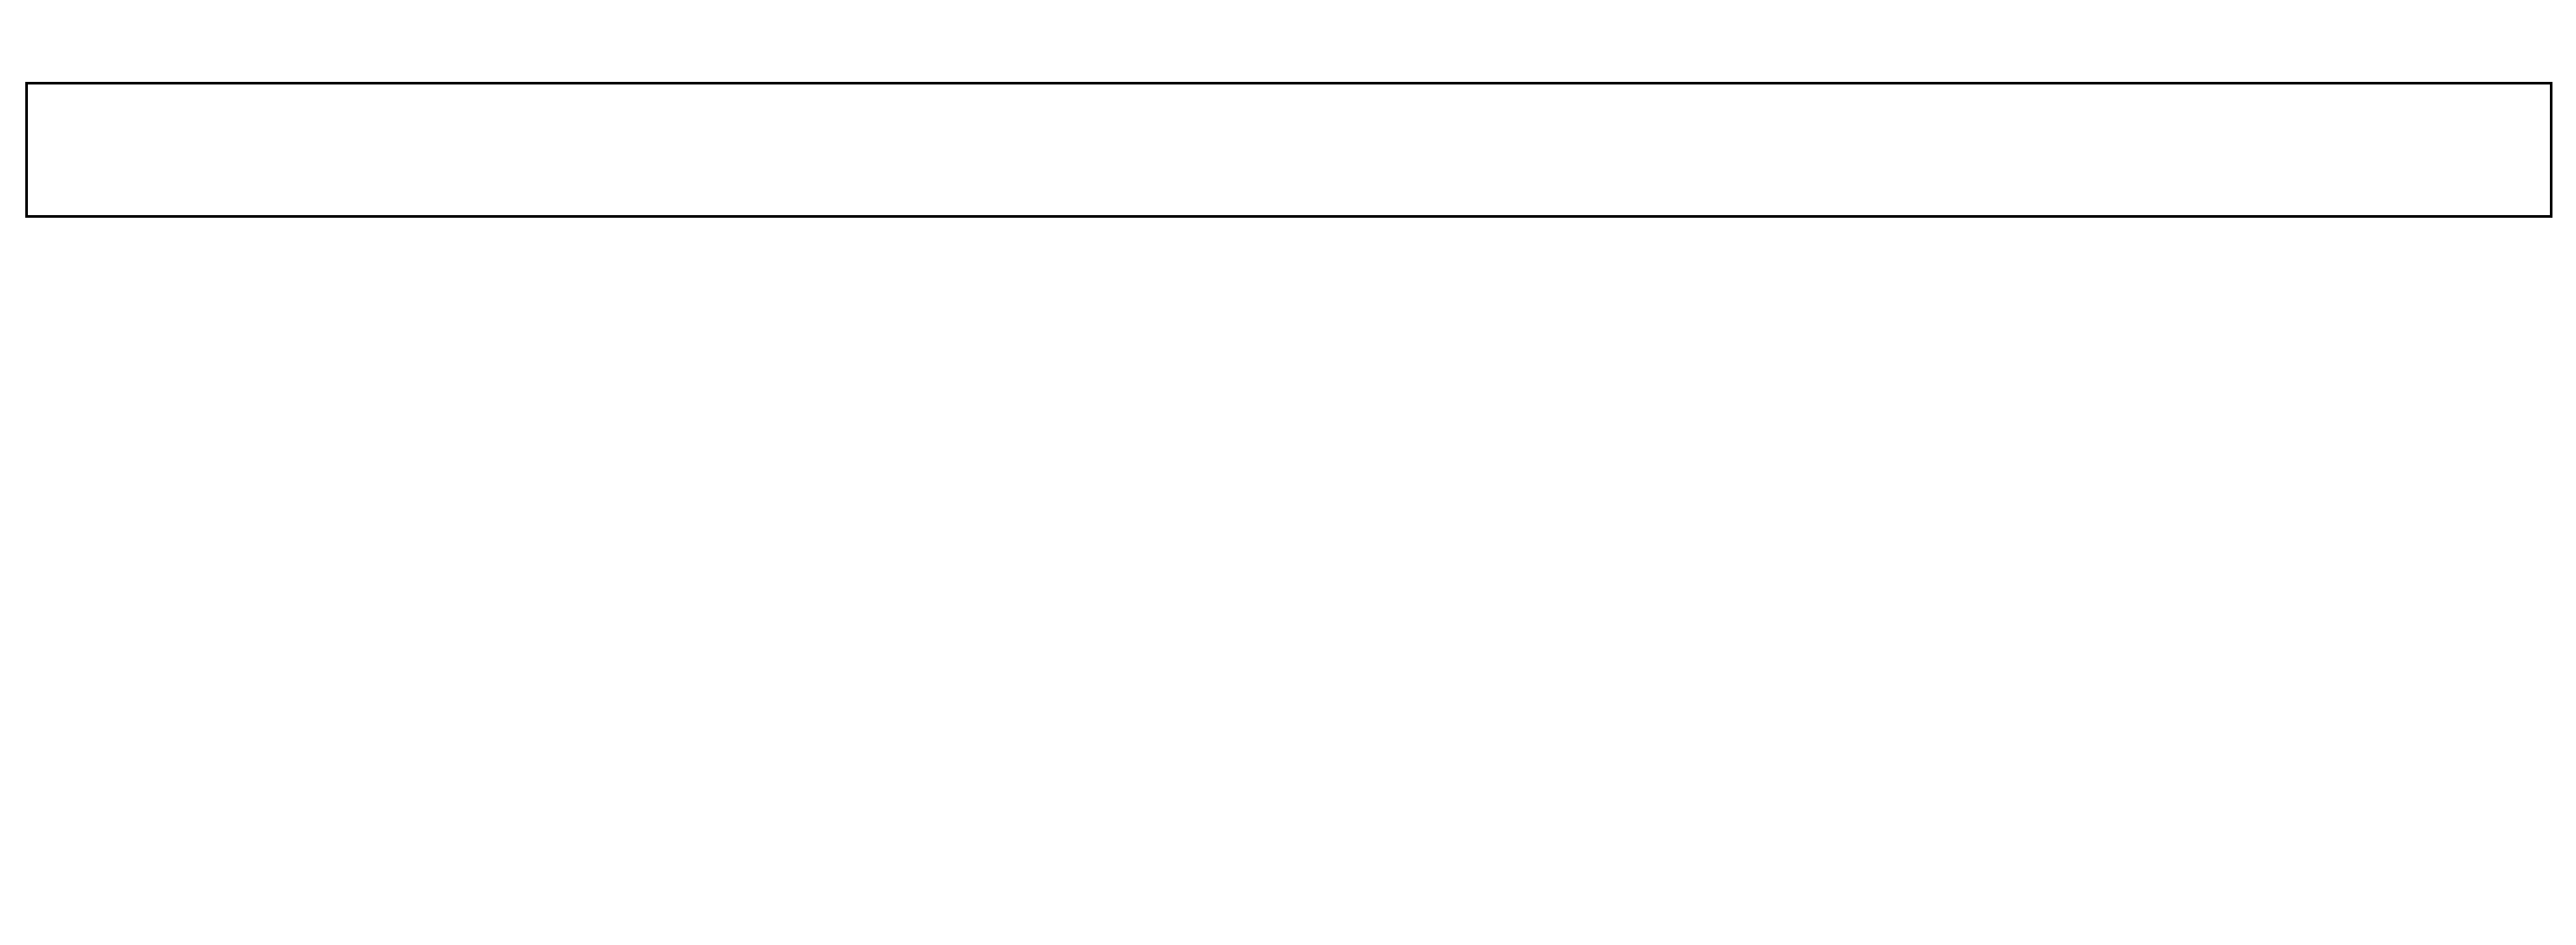
\includegraphics[width=0.8 \textwidth]{figs/RISC-V/指令表示/R_I.eps}
%   \caption{I型指令就是把R型指令的前两个域合并成一个了12位的有符号数}
%   \label{fig:R_I} %设置图形引用名称
% \end{figure}



\subsubsection{S指令与B指令}
\textbf{S指令}是用于写存储器的。

\textbf{B指令}是用于分支转移操作的,其实本质上是S指令的一个变体,之前也叫\textbf{SB指令}

\subsubsection{U指令和J指令}
\textbf{U指令}用于高20-bit位立即数操作。

\textbf{J指令}是用于跳转操作,其实是U指令的一个变体,之前也叫\textbf{UJ指令}


\subsection{流水线}
\subsubsection{处理器性能度量方法}
首先,我认为在我们研究之前应该明确我们常说的提高性能是指什么,是表示更快的响应时间?从而更快的完成需要执行的任务?还是单位时间内能完成更多的任务?还是使用寿命更长一些?

我觉得性能的本质是——处理器干起活来利不利索,如公式(\ref{eq:Computer_Analogy})是与处理器性能有关的定理。

\begin{equation}\label{eq:Computer_Analogy}
    \frac{ Time }{ Program } = \frac{ Instructions }{ Program } * \frac{ Cycles }{ Instruction } * \frac{ Time }{ Cycle }
\end{equation}

\subsubsection{结构冒险}
本质上讲造成出现结构冒险的原因就是因为在硬件层面上是不支持同一周期来执行多条指令的。

但出现这个结构冒险,也比较好解决,既然是硬件层面的问题,那就从硬件的方向来入手解决 1. 让其他阻塞一下等待硬件空闲下来在使用,2. 要么就是多添加点硬件。


\subsubsection{数据冒险}
导致数据冒险发生简言之就是不同指令之间存在\textbf{数据的关联},造成了无法提供指令执行所需的数据,进而指令不能在预期的时钟周期内执行。

解决方案就是 1.让其他阻塞一会儿等待数据使用完在继续使用;2.增加一个\textbf{旁路(bypassing)},
这样的好处就是不需要浪费时间等指令执行完成就可以立即解决数据冒险。如图\ref{fig:Data_Hazards1} 所示,第一条add指令执行EX阶段的输出前递到sub指令的EX阶段的输入,替换sub指令在第二阶段督促的寄存器X1的值,这样就很好的解决了数据冒险。

\begin{figure}[htbp]
    \centering
    \def\svgwidth{\columnwidth}
    \import{./figs/RISC-V/流水线/数据冒险/数据冒险1/}{数据冒险1.pdf_tex}
    \caption{这张图片就显示了旁路的效果}
    \label{fig:Data_Hazards1}
\end{figure}
% \begin{figure}[htbp]
%   \centering %居中显示
%   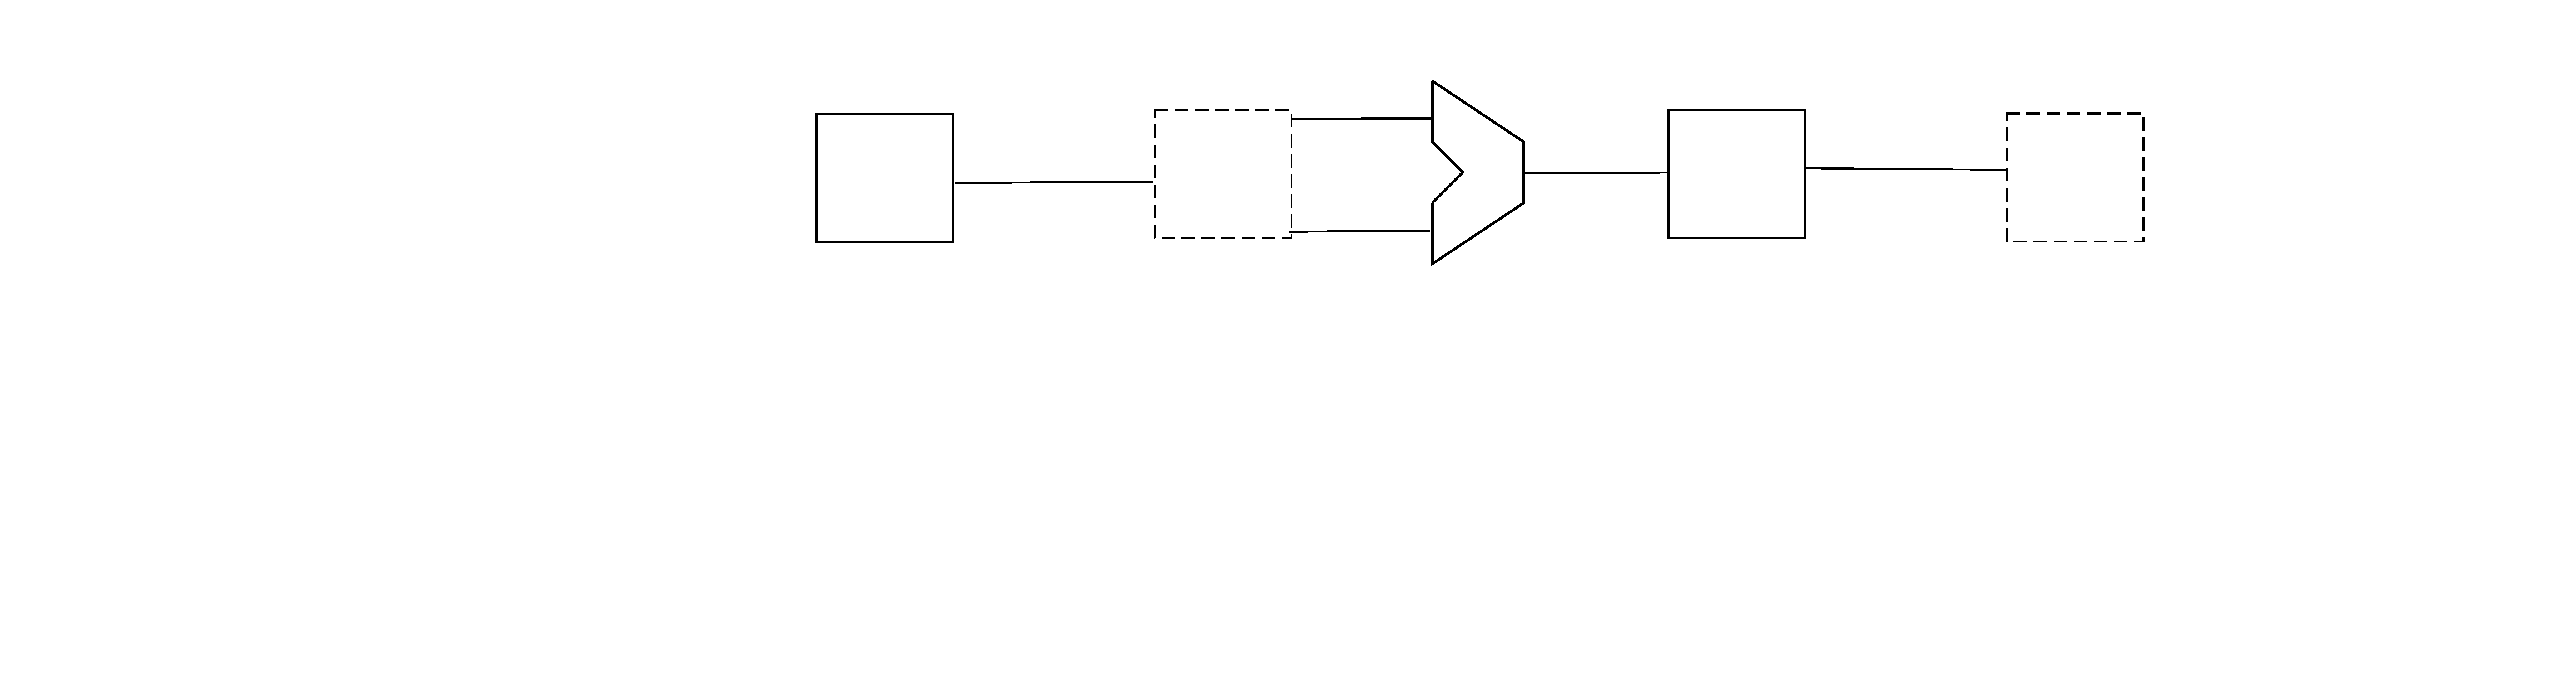
\includegraphics[width=0.8 \textwidth]{figs/RISC-V/流水线/数据冒险1.eps}
%   \caption{这张图片就显示了旁路的效果}
%   \label{fig:Data_Hazards1} %设置图形引用名称
% \end{figure}

旁路看起来挺完美的,好像只需要加上一条新的电路,这样就可以节省出那么多的时间,然后利用这省出的时间可以完成更多的指令,这听起来的确太完美了,但是现实往往让人比较无奈,有时尽管已经使用了旁路,还是会出现不可避免的需要\textbf{流水线停顿(pipeline Stall)},俗称\textbf{气泡(bubble)},图\ref{fig:Data_Hazards2}就是在 load 指令执行之后,紧跟着一条需要使用他结果的 R 型指令,可惜 R 指令需要到执行运算的时候才需要上一条 load 指令的值,所以这里就只能添加 bubble 来等待。

\begin{figure}[htbp]
    \centering
    \def\svgwidth{\columnwidth}
    \import{./figs/RISC-V/流水线/数据冒险/数据冒险2/}{数据冒险2.pdf_tex}
    \caption{这张就表示有时即使使用旁路,也许要阻塞等待}
    \label{fig:Data_Hazards2}
\end{figure}
% \begin{figure}[htbp]
%   \centering %居中显示
%   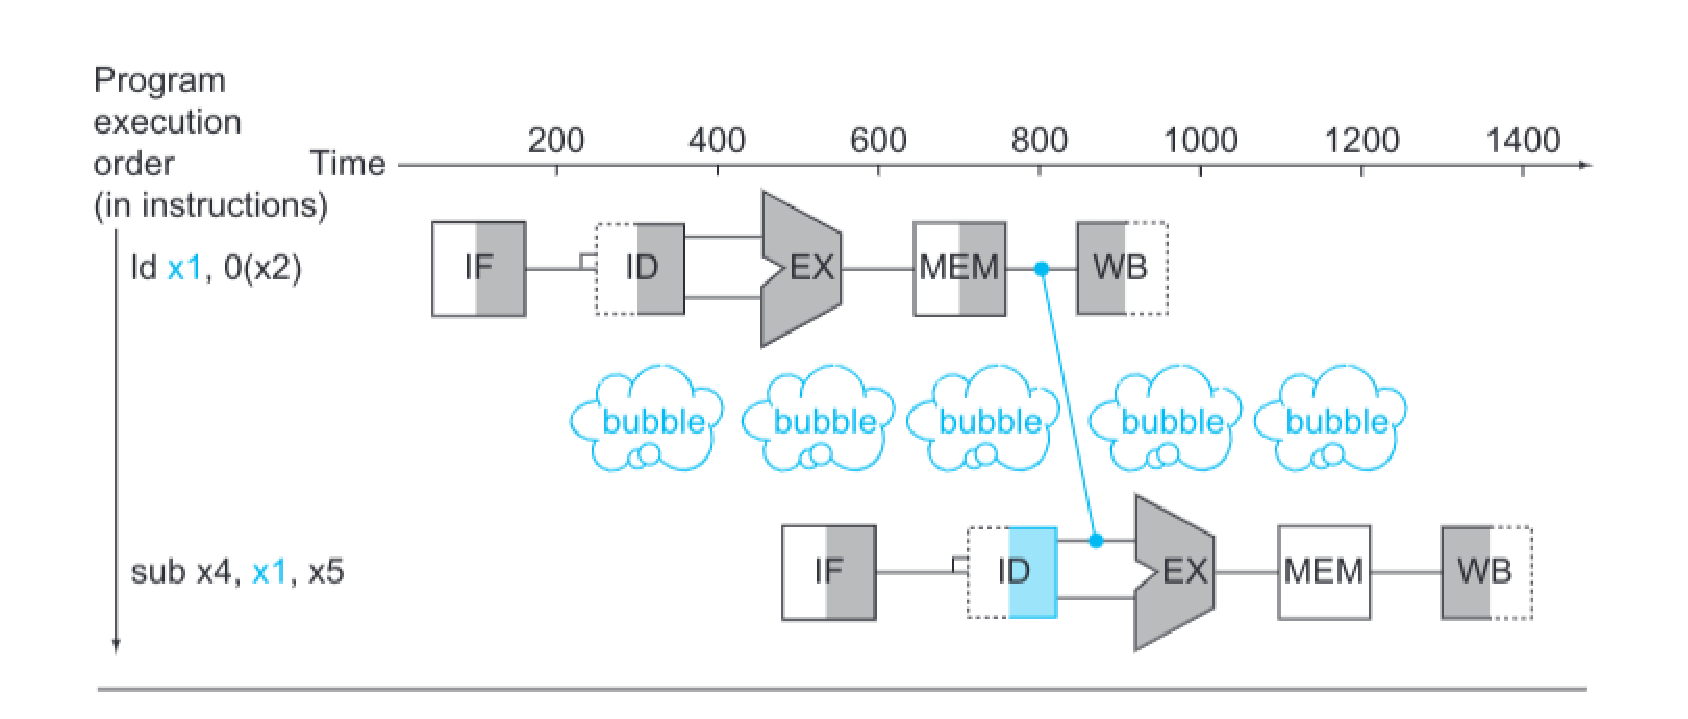
\includegraphics[width=0.8 \textwidth]{figs/RISC-V/流水线/数据冒险2.eps}
%   \caption{这张就表示有时即使使用旁路,也许要阻塞等待}
%   \label{fig:Data_Hazards2} %设置图形引用名称
% \end{figure}


\subsubsection{控制冒险}
这种冒险发生在根据一条指令的结果判断接下来要执行的分支程序。如图\ref{fig:Control_Hazards}所示

\begin{figure}[htbp]
  \centering %居中显示
  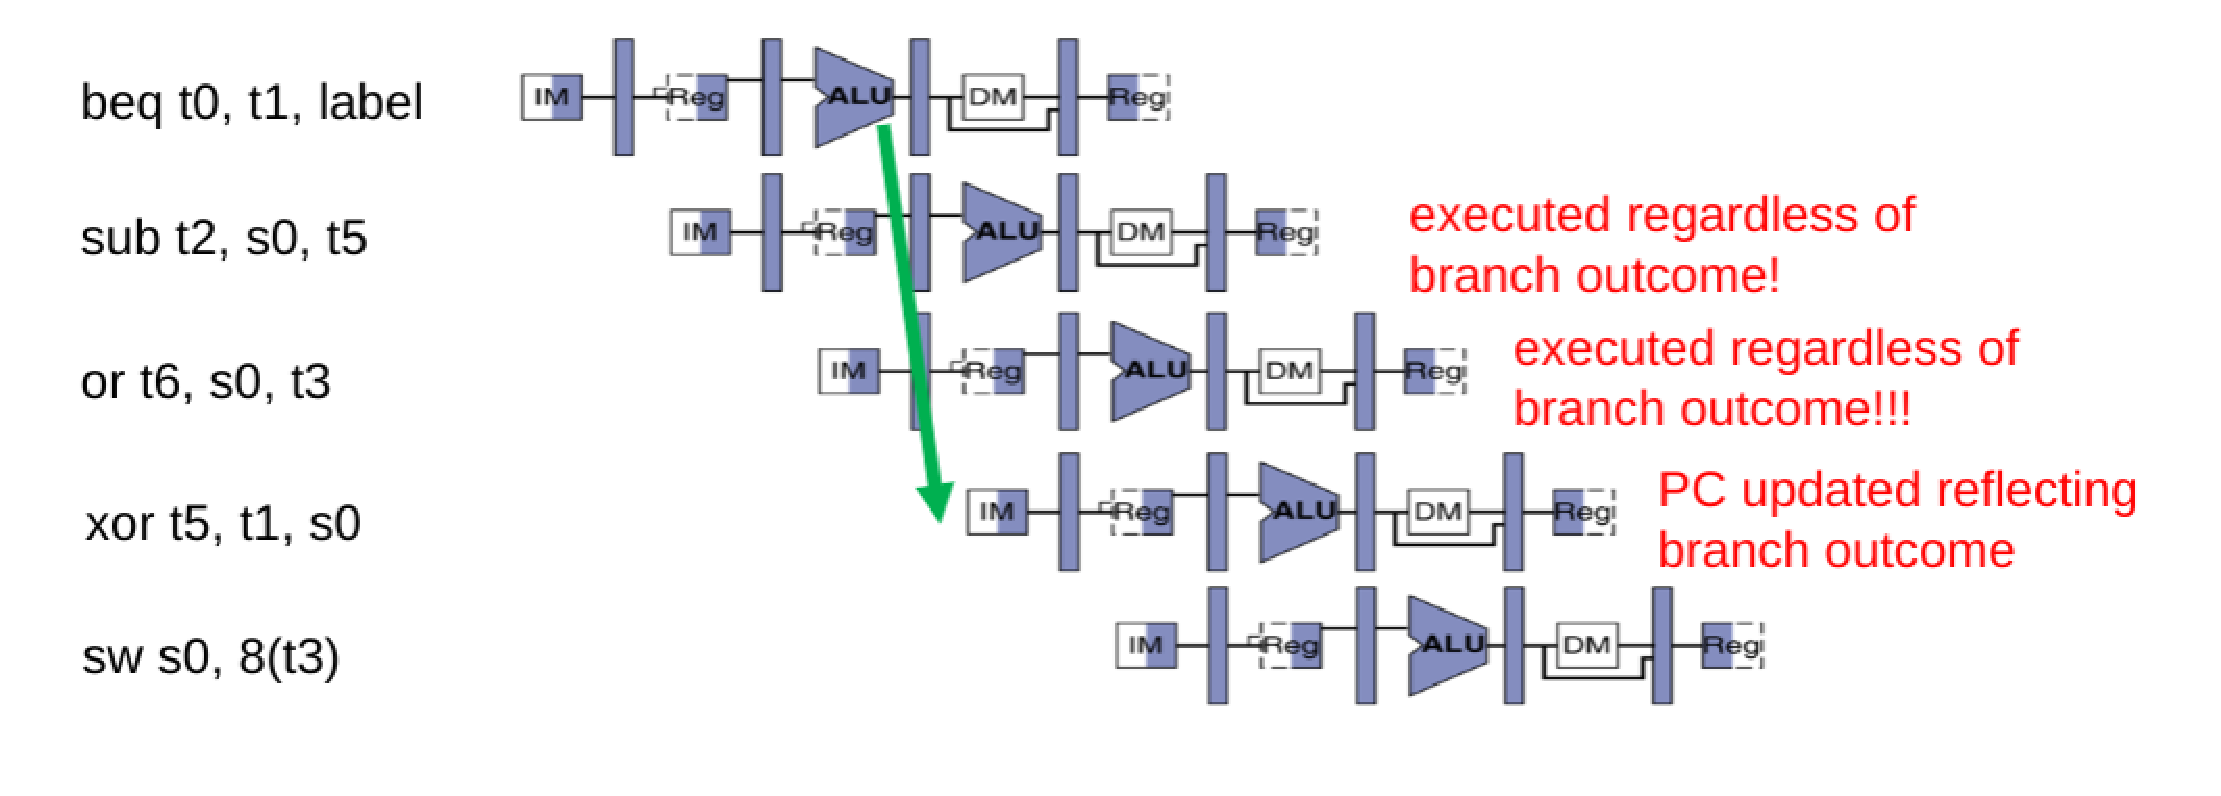
\includegraphics[width=0.8 \textwidth]{figs/RISC-V/流水线/控制冒险.eps}
  \caption{控制冒险}
  \label{fig:Control_Hazards} %设置图形引用名称
\end{figure}

解决方法1.阻塞等待,2.采用\textbf{分支预测},要是预测对了,就继续执行,如图\ref{fig:Control_Hazards_Success};如果预测错了,流水线清空刚才加载错误的指令,重新在装载正确的指令,如图\ref{fig:Control_Hazards_Fail}。

\begin{figure}[htbp]
  \centering %居中显示
  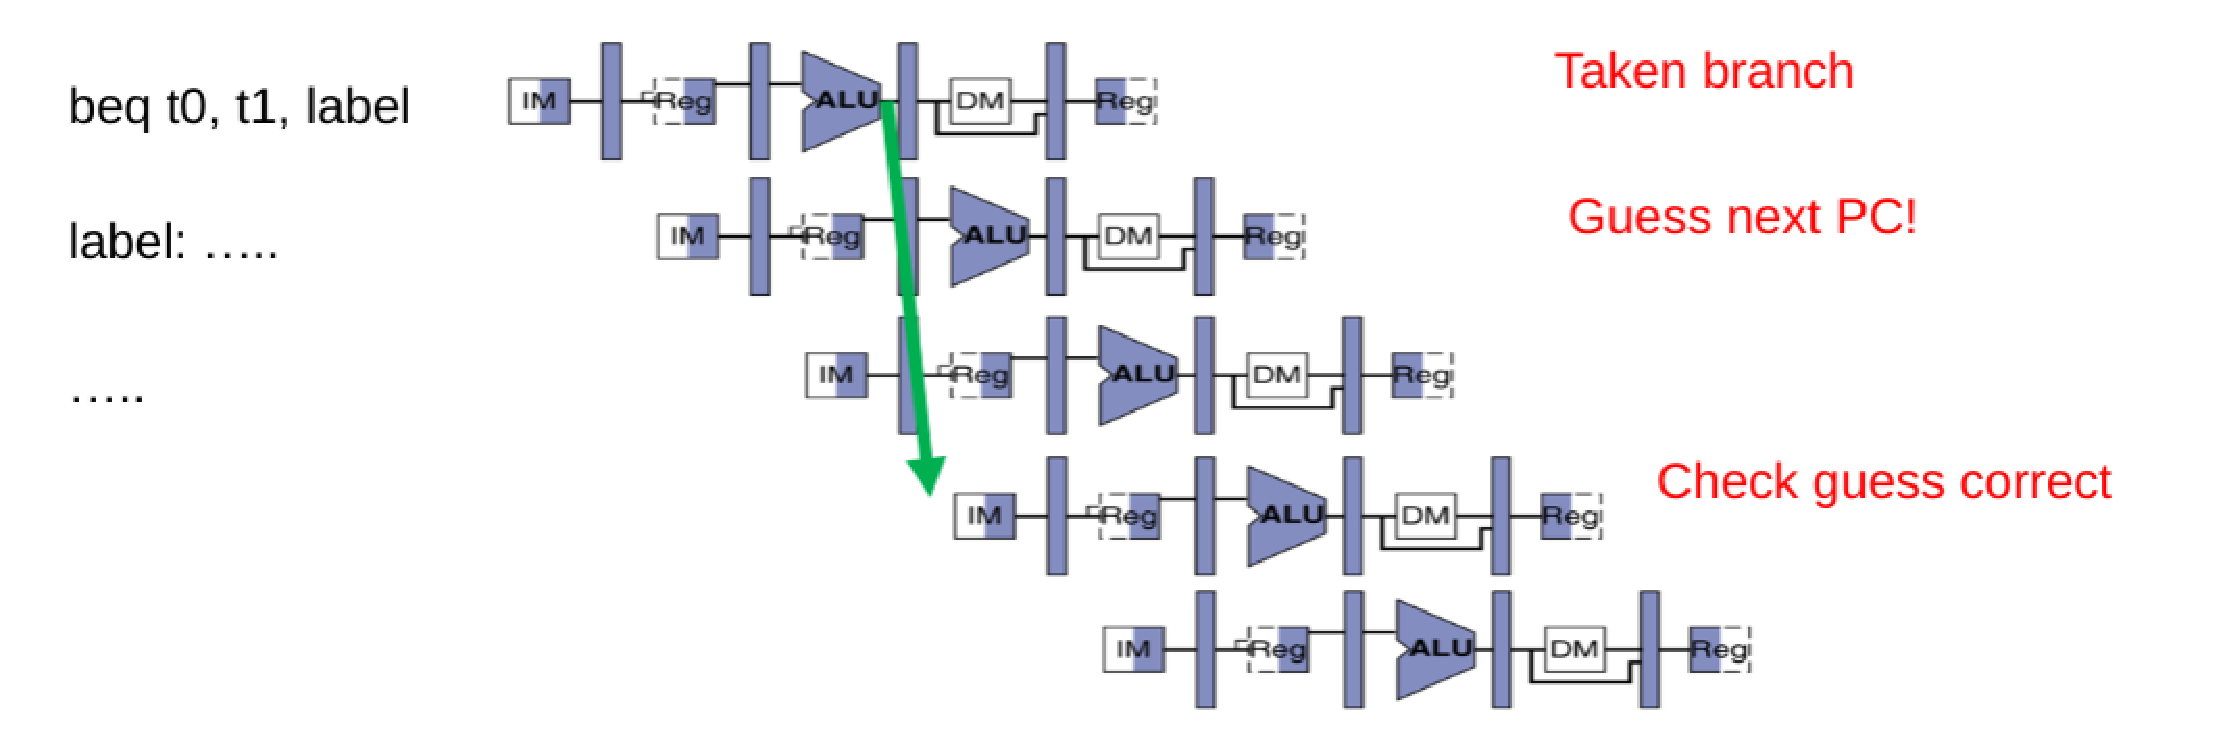
\includegraphics[width=0.8 \textwidth]{figs/RISC-V/流水线/控制冒险_预测成功.eps}
  \caption{分支预测:预测成功}
  \label{fig:Control_Hazards_Success} %设置图形引用名称
\end{figure}

\begin{figure}[htbp]
  \centering %居中显示
  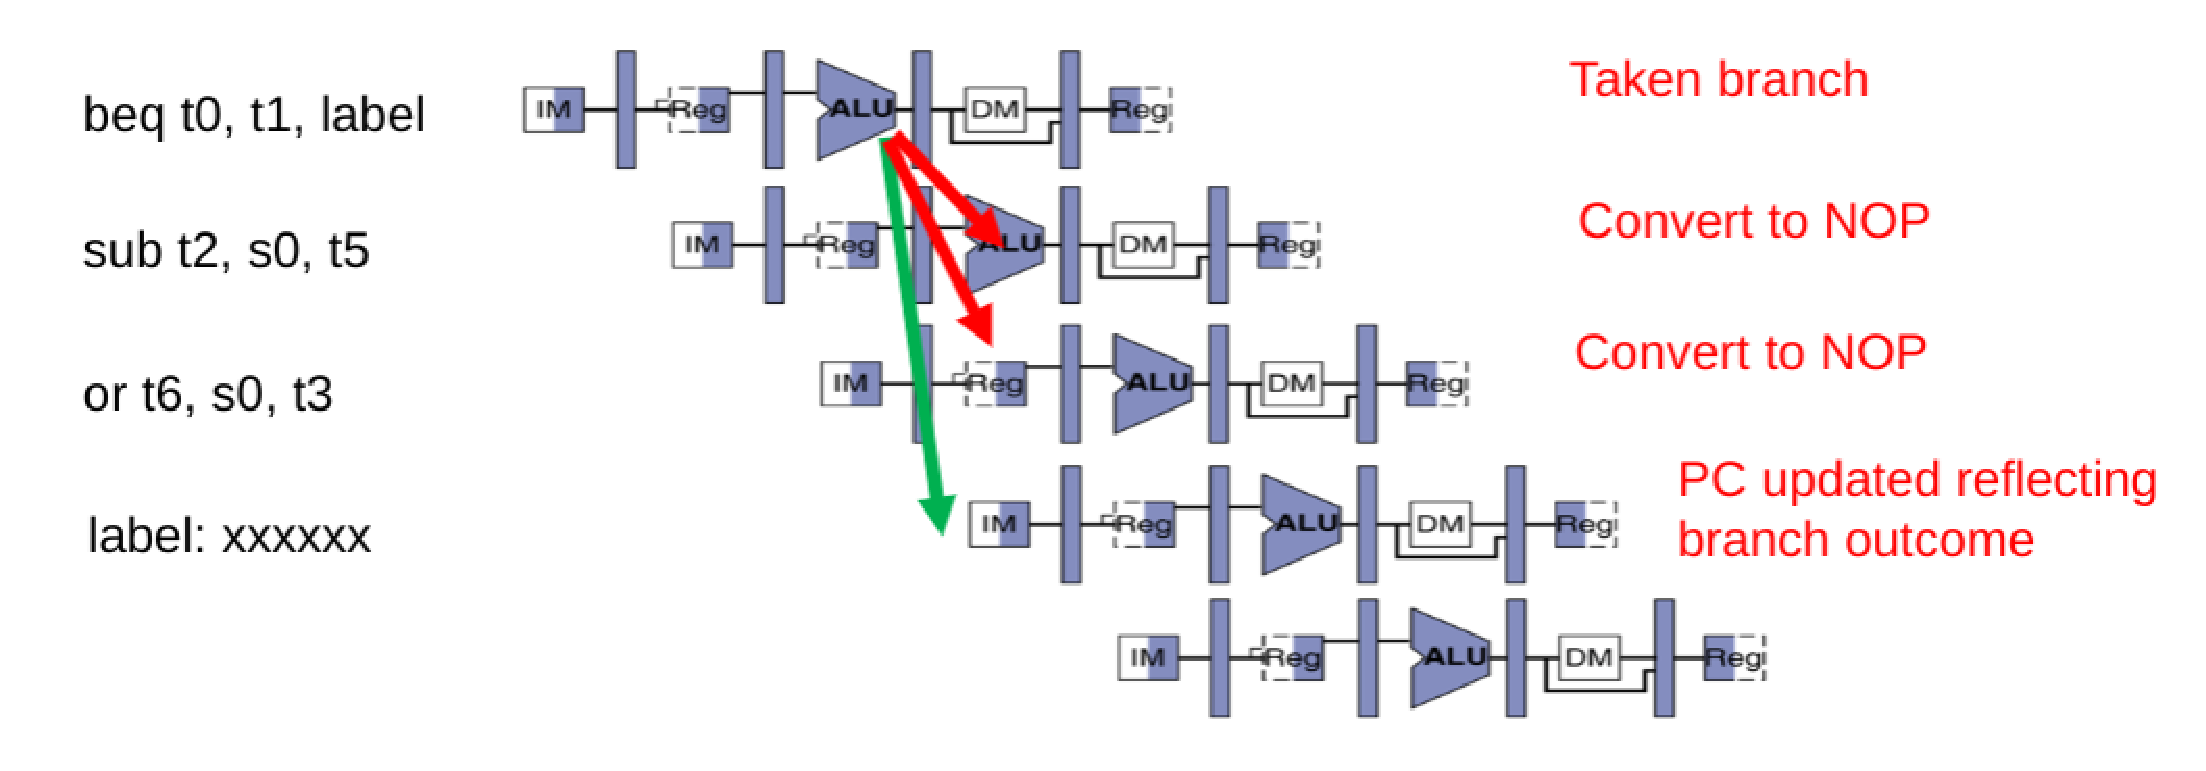
\includegraphics[width=0.8 \textwidth]{figs/RISC-V/流水线/控制冒险_预测失败.eps}
  \caption{分支预测:预测失败}
  \label{fig:Control_Hazards_Fail} %设置图形引用名称
\end{figure}







